\subsection{NLP and VerbNet as a Computational Lexical Resource}\label{nlp}
Natural language processing (NLP) is a computational method for the automated analysis and representation of human language \cite{cambria2014jumping}. NLP techniques offer potential advantages to improve the quality of USs and can be used to parse, extract, or analyze US's data. It has been widely used to help in the software engineering domain (\emph{e.g.}, managing software requirements \cite{Arias2018}, extraction of actors and actions in requirement document \cite{al2018use}.

NLP techniques are usually used for text preprocessing (\emph{e.g.}, tokenization, \emph{Part-of-Speech} (POS) tagging, and dependency parsing). Several NLP approaches can be used (\emph{e.g.}, syntactic representation of text and computational models based on semantic features). Syntactic methods focus on word-level approaches, while the semantic focus on multiword expressions \cite{cambria2014jumping}.

A computational lexicon resource is a systematically organized repository of words or terms, complete with linguistic and semantic data. These lexicons play a pivotal role in facilitating NLP systems focused on semantic analysis by offering comprehensive insights into language elements, encompassing word forms, part-of-speech (POS) categories, phonetic details, syntactic properties, semantic attributes, and frequency statistics. Lexical classes, defined in terms of shared meaning components and similar (morpho-) syntactic behaviour of words, have attracted considerable interest in NLP \cite{cambria2014jumping}. These classes are useful for their ability to capture generalizations about a range of (cross-) linguistic properties. NLP systems can benefit from lexical classes in a number of ways. As the classes can capture higher level abstractions (\emph{e.g.} syntactic or semantic features) they can be used as a principled means to abstract away from individual words when required. Their predictive power can help compensate for lack of sufficient data fully exemplifying the behaviour of relevant words \cite{kipper2006extending}.

Upon the completion of the transformation of USs utilizing a Conditional Random Fields (CRF) approach, wherein entities, actions (both primary and secondary), persona, and their relational attributes (specifically, triggers, targets and contains) are meticulously annotated and structured as a graph-based representation, a preliminary imperative emerges. This imperative entails the determination of a representative semantic interpretation for the ascertained actions. This determination, in turn, serves as a prerequisite for the generation of corresponding transformation rules, namely, \enquote{create}, \enquote{delete}, \enquote{preserve} and \enquote{forbidden} rules.

The attainment of this representative semantic interpretation hinges upon the application of a suite of foundational lexical resource techniques of a conceptual nature. These techniques assume a pivotal role in furnishing the essential cognitive infrastructure, facilitating a comprehensive grasp of the semantic roles, syntactic characteristics, and the systematic categorization to \enquote{creation}, \enquote{deletion}, \enquote{preservation} and \enquote{forbiddance} of linguistic elements embedded within the construct of the US.
\subsection*{VerbNet} \label{verbnet}
VerbNet (VN) is a hierarchical domain-independent, broad-coverage verb lexicon with mappings to several widely-used verb resources, including WordNet \cite{miller1995wordnet}, Xtag \cite{prolo2002generating}, and FrameNet \cite{baker1998berkeley}. It includes syntactic and semantic information for classes of English verbs derived from Levin’s classification, which is considerably more detailed than that included in the original classification. 

Each verb class in VN is completely described by a set of members, thematic roles for the predicate-argument structure of these members, selectional restrictions on the arguments, and frames consisting of a syntactic description and semantic predicates with a temporal function, in a manner similar to the event decomposition of Moens and Steedman \cite{moens2005temporal}. The original Levin classes have been refined, and new subclasses added to achieve syntactic and semantic coherence among members.
\subsection*{Syntactic Frames}
Semantic restrictions, such as constraints related to animacy, humanity, or organizational affiliation, are employed to limit the types of thematic roles allowed within these classes. Furthermore, each syntactic frame may have constraints regarding which prepositions can be used. 

Additionally, there may be additional constraints placed on thematic roles to indicate the likely syntactic nature of the constituent associated with that role.
Levin classes are primarily characterized by NP (noun phrase) and PP (prepositional phrase) complements. 

Some classes also involve sentential complementation, albeit limited to distinguishing between finite and non-finite clauses. This distinction is exemplified in VN, particularly in the frames for the class Tell-37.2, as shown in Examples (1) and (2), to illustrate how the differentiation between finite and non-finite complement clauses is implemented.
\begin{enumerate}
\item Sentential Complement (finite): \\ \ \ \enquote{Susan told Helen that the room was too hot.} \\ \emph{Agent V Recipient Topic [+sentential – infinitival]}
\item Sentential Complement (nonfinite): \\ \ \  \enquote{Susan told Helen to avoid the crowd.}\\ \emph{Agent V Recipient Topic [+infinitival – wh\_inf]}
\end{enumerate}
\subsection*{Semantic Predicates}
Each VN frame also contains explicit semantic information, expressed as a conjunction of Boolean semantic predicates such as \enquote{motion}, \enquote{contact}, or \enquote{cause}. Each of these predicates is associated with an event variable E that allows predicates to specify when in the event the predicates are true $start(E)$ for preparatory stage, $during(E)$ for the culmination stage, and $end(e)$ for the consequent stage). 

Relations between verbs (or classes) such as antonymy and entailment present in WordNet and relations between verbs (and verb classes) such as the ones found in FrameNet can be predicted by semantic predicates. Aspect in VN is captured by the event variable argument present in the predicates.
\subsection*{The VerbNet Hierarchy}
VerbNet represents a hierarchical structure of verb behaviour, with groups of verb classes sharing similar semantics and syntax. Verb classes are numbered based on common semantics and syntax, and classes with the same top-level number (e.g., 9-109) have corresponding semantic relationships. 

For instance, classes related to actions like \enquote{putting}, such as \enquote{put-9.1}, \enquote{put\_spatial-9.2}, \enquote{funnel-9.3}, all belong to class number 9 and relate to moving an entity to a location. Classes sharing a top class can be further divided into subclasses, as seen with \enquote{wipe} verbs categorized into \enquote{wipe\_manner} $(10.4.1)$ and \enquote{wipe\_inst} $(10.4.2)$ specifying the manner and instrument of \enquote{wipe} verbs in the \enquote{Verbs of Removing} group of classes (class number 10).

The classification encompasses class numbers 1-57, derived from Levin's classification \cite{levin1993english}, and class numbers 58-109, developed later by Korhonen and Briscoe \cite{korhonen2004extended}. The later classes are more specific, often having a one-to-one relationship between verb type and verb class. This hierarchical structure helps categorize and organize verbs based on their semantic and syntactic properties.
\subsection*{Verb Class Hierarchy Contents}
Each individual verb class within VerbNet is hierarchical. These classes can include one or more \enquote{subclasses} or \enquote{child} classes, as well as \enquote{sister} classes. All verb classes have a top-level classification, but some provide further specification of the behaviours of their verb members by having one or more subclasses. 

Subclasses are identified by a dash followed by a number after the class information. For example, the top class might be \enquote{spray-9.7}, and a subclass would be denoted as \enquote{spray 9.7-1}. This hierarchy allows for a more detailed and structured organization of verb behaviour within VerbNet. 
\begin{itemize}
\item \textbf{Top Class:} The highest class in the hierarchy; all features in the top class are shared by every verb in the class. The top class of the hierarchy consists of syntactic constructions and semantic role labels that are shared by all verbs in this class.
\item \textbf{Parent Class:} Dominates a subclass; all features are shared with subordinate classes.
\item \textbf{Subclasses:} VerbNet subclasses inherit features from the top class but specify further syntactic and semantic commonalities among their verb members. These can include additional syntactic constructions, further selectional restrictions on semantic role labels, or new semantic role labels.
\item \textbf{Child Class:} Is dominated by a parent class; inherits features from this parent class, but also adds information in the form of additional syntactic frames, thematic roles, or restrictions. 
\item \textbf{Sister Class:} A subclass directly dominated by a parent class. This parent class also, directly dominates another subclass, so the two subclasses are sisters to one another. Sister classes do not share features.
\end{itemize}
Figure \ref{fig:hierachy_class} illustrate an example of class hierarchy from spray-9.7 class.
\begin{figure}[h]
\center
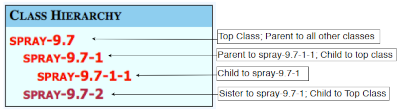
\includegraphics[scale=0.5]{Class_hierarchy_for_spray-9_punk_7_class}
\caption{Class hierarchy for spray-9.7 class \cite{heck2014quality}}\label{fig:hierachy_class}
\end{figure}
Verb Classes are numbered according to shared semantics and syntax, and classes which share a top-level number (9-109) have corresponding semantic relationships. 

For instance, verb classes related to putting, such as put-9.1, put\_spatial-9.2, funnel-9.3, etc. are all assigned to the class number 9 and related to moving an entity to a location. 

Classes that share a top class can also be divided into subclasses, such as wipe verbs in wipe\_manner (10.4.1) and wipe\_inst (10.4.2) which specify the manner and instrument of wipe verbs in the \enquote{Verbs of Removing} group of classes (class number 10). 

An example of top-class numbers and their corresponding types is given in Table \ref{tb:vtype_example}. Class numbers 1-57 are drawn directly from Levin's (1993) classification. Class numbers 58-109 were developed later in the work of Korhonen \& Briscoe (2004). Notably, the verb types of the later classes are less general, as indicated by the fact that most of these classes have a one-to-one relationship between verb type and verb class.

\begin{figure}[h]
\begingroup
\scriptsize
\centering
\begin{tabularx}{12cm}{l  l  l}
\hline
Class Number	&Verb Type	&Verb Class \\
\hline 
\hline
10&	Verbs of Removing		&banish-10.2 \\
&&cheat-10.6.1\\
&&clear-10.3\\
&&debone-10.8\\
&&fire-10.10\\
&&mine-10.9\\
&&pit-10.7\\
&&remove-10.1\\
&&resign-10.11\\
&&steal-10.5\\
&&wipe\_manner-10.4.1\\
\hline
26	&Verbs of Creation and Transformation	&adjust-26.9 \\
&&build-26.1 \\
&&convert-26.6.2\\
&&create-26.4\\
&&grow-26.2.1\\
&&knead-26.5\\
&&performance-26.7\\
&&rehearse-26.8\\
&&turn-26.6.1\\
\hline
13&	Verbs of Change of Possession	&berry-13.7 \\
&&contribute-13.2\\
&&equip-13.4.2\\
&&exchange-13.6.1\\
&&fulfilling-13.4.1\\
&&future\_having-13.3\\
&&get-13.5.1\\
&&give-13.1\\
&&hire-13.5.3\\
&&obtain-13.5.2\\
\hline
\end{tabularx}

\captionof{table}{An example of top-class numbers and their corresponding verb-type\cite{verbnet_guidelines}}\label{tb:vtype_example}

\endgroup
\end{figure}
\subsection*{Conclusion}\label{nlp_bottom_line}
The methodological categorisation of verbs into hierarchical classes in VerbNet provides a structured and all-encompassing framework for understanding verb behaviour. This alignment with our project goals is of utmost importance as it supports our task of formulating transformation rules based on semantic interpretations of the actions (verbs) recognised by CRF and described in USs. VerbNet's organisational structure fits seamlessly with the requirements of our project and ensures the necessary precision and granularity that is essential for our semantic analysis and rule generation.
\subsection{Analysis by Graph Transformation Tool}\label{gts}
In this section, some basic definitions about graph transformation and transformation rules are first established for better understanding. Afterwards, we dive into graph transformation tools, which play a pivotal role in our methodology.

In a software development process, the class architecture is getting changed over the development, \emph{e.g.} due to a change of requirements, which results in a change of the class diagram. During runtime of a software, an object diagram can also be modified trough creating or deleting of new objects.

Many structures, that can be represented as graph, are able to change or mutate. This suggests the introduction of a method to modify graphs through the creation or deletion of nodes and edges. This graph modification can be performed by the so-called graph transformations. There are many approaches to model graph transformations \emph{e.g.} the double pushout approach or the single pushout approach, which are both concepts based on pushouts from category theory in the category Graphs.
\subsection*{Graphs and Typed Graphs}
A graph consists of nodes and edges, with each edge connecting precisely two nodes and having the option to be directed or undirected. When an edge is directed, it designates a distinct start node (source) and an end node (target). For the purpose of this discussion, we will focus on directed graphs.

\begin{definition}[\textbf{graph}]
\label{def_graph}
A \emph{graph} $G = (V,E,s,t)$ contains $V$, a set of nodes, $E$, a set of edges, $s: E \to V$, a source function, where $s(e)$ is the start node of $e \in E$ and a target function $t:E \to V$, where $t(e)$ is the end node of a edge $e \in E$.
\end{definition}

\begin{definition}[\textbf{Transformation Rule}]
A \emph{transformation rule} denotes which nodes and edges of a graph have to be deleted and which nodes and edges have to be created.
In the double-pushout approach a transformation rule $p = L \xhookleftarrow{l} K \xhookrightarrow{r} R$ consists of three graphs $L,K,R$, two graph morphisms $l: K \to L$ and $r: K \to R$, where $K$ contains all elements, that remain in the graph, $L \setminus l(K)$ contains the elements that are removed and $R \setminus r(K)$ contains the elements, that are created.
\end{definition}
\begin{definition}[\textbf{Graph Transformation}]
In the context of \emph{graph transformations}, when we have two graphs $G$ and $H$, along with a transformation rule $p$, we can apply this rule to graph $G$ at match $m$. This application, denoted as $G \xRightarrow{p,m} H$, results in graph $H$. The match, represented as $m : L \hookrightarrow G$, is an injective graph morphism, and $L$ contains all the nodes and edges of $p$ that remain intact and are not deleted during the transformation.
\end{definition}
As outlined in Section \ref{dmodel}, where we elucidated our utilization of Conditional Random Fields (CRF) as a graph-based metamodeling and compositional approach for annotating USs, each US is meticulously structured and annotated in the form of a graph. Subsequently, we will apply transformation rules to these CRF-generated graphs to modelling graph transformation.

To accomplish this objective, we have harnessed the capabilities of established lexical resources such as VerbNet. This utilization of VerbNet enables us to categorize actions (which are verbs) extracted from the US into three distinct categories, namely: \enquote{create}, \enquote{delete}, \enquote{forbid}. These categories serve as essential components of transformation rules that articulate precise changes within the graph-based representation. 
\subsection*{Henshin: A Tools for In-Place EMF Model Transformations}\label{henshin}
The Eclipse Modelling Framework (EMF) provides modelling and code generation facilities for Java applications based on structured data models. Henshin is a language and associated tool set for in-place transformations of EMF models. 

The Henshin transformation language uses pattern-based rules on the lowest level, which can be structured into nested transformation units with well-defined operational semantics. So-called amalgamation units are a special type of transformation units that provide a forall-operator for pattern replacement. For all of these concepts, Henshin offers a visual syntax, sophisticated editing functionalities, execution and analysis tools. The Henshin transformation language has its roots in attributed graph transformations, which offer a formal foundation for validation of EMF model transformations \cite{arendt2010henshin}.
\subsection*{Graph Types}
Graph transformation-based approaches, essentially define model transformations using rules consisting of a pre-condition graph, called the left-hand side (LHS), and a post-condition graph, called the right-hand side (RHS) of the rule. Informally, the execution of a model transformation requires that a matching of objects in the model (host graph) to the nodes and edges in the LHS is found, and these matched objects are changed in such a way that the nodes and edges of the RHS match these objects \cite{tichy2013detecting}.

The performance of graph transformation-based model transformations is mainly determined by the efficiency of the match finding of the LHS. Consequently, model transformation languages offer different options to add constraints to the LHS of model transformations to improve the performance of the matching \cite{tichy2013detecting}. To be efficient, graph transformation tools usually employ heuristics such as search plans to provide good performance (e.g. \cite{varro2012algorithm}).
\subsection*{Structure and Application of Rules}
The Henshin transformation language is defined by means of a metamodel. The Henshin metamodel is closely aligned to the underlying formal model of double pushout (DPO) graph transformations \cite{tichy2013detecting}. Thus, rules consist of a left-hand side and a right-hand side graph as instances of the \emph{Graph} class. Rules further contain node mappings between the LHS and the RHS which are omitted here for better readability. Graphs consist of a set of Nodes and a set of Edges. Nodes can additionally contain a set of Attributes. These three kinds of model elements are typed by their corresponding concepts in the Ecore metamodel of EMF.
\subsection*{Application Conditions}
To conveniently determine where a specified rule should be applied, application conditions can be defined. An important subset of application conditions is negative application conditions (NACs) which specify the non-existence of model patterns in certain contexts.
In the Henshin transformation model, graphs can be annotated with application conditions using a \emph{Formula}. This formula is either a logical expression or an application condition, which is an extension of the original graph structure by additional nodes and edges. A rule can be applied to a host graph only if all application conditions are fulfilled \cite{arendt2010henshin}.
\subsection*{Attribute and Parameters}
Nodes may also include a set of Attributes. Rules inherit from Units and can thus include various Parameters. A common use of parameters is to transmit an Attribute value (such as a name) from a node to be matched in the rule. To restrict the application of a rule, the metamodel encompasses concepts for representing nested graph conditions \cite{habel2009correctness} as well as attribute conditions.
\subsection*{State Space Exploration}
Henshin support in-place model transformation, Arendt et al. have developed a state space generation tool, which allow to simulating all possible executions of a transformation for a given input model, and to apply model checking, similar to the GROOVE \cite{kastenberg2006model} tool. Henshin can generate finite as well as large state space exploration. Regarding generation and analysis of large state space, the tool’s ability to utilize parallel algorithms, taking advantage of modern multi-core processors, which enables the handling of state spaces with millions of states. 
\subsection*{Analyzing Conflicts and Dependencies}
The elements that comprise the system under construction interact with each other, establishing dependencies among them \cite{kastenberg2006model}. In Figure \ref{fig:inherited_dependencies}, \emph{element A} requires \emph{element B}, generating a dependency between them. Such dependencies are naturally inherited by the USs ($US_i$ 
cannot be implemented until $US_j$ is implemented). 

Therefore, the natural dependencies between USs should be accepted as inevitable. In fact, only a fifth of the requirements can be considered with no dependencies \cite{carlshamre2001industrial}. The existence of dependencies between USs makes it necessary to have some implemented before others \cite{carlshamre2001industrial},\cite{Greer2004},\cite{logue2008handling}. If the order of USs implementation does not consider these dependencies, it may have a large number of preventable refactorings, increasing the total cost of the project needlessly. Identifying beforehand the dependencies increases the ability to effectively deal with changes. 

Hence, light systematic mechanisms are needed to help identify dependencies between USs \cite{gomez2010systematic}.
\begin{figure}[h]
\center
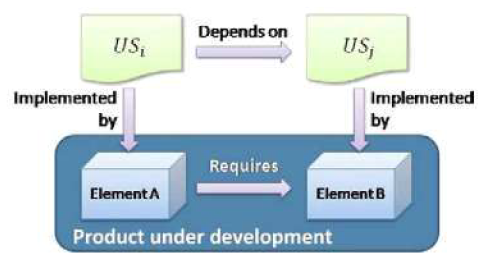
\includegraphics[scale=0.7]{inherited_depencendy}
\caption{  Inherited dependencies by user stories\cite{gomez2010systematic} }\label{fig:inherited_dependencies}
\end{figure}
The critical pair analysis (CPA) for graph rewriting \cite{hartmanis2006monographs} has been adapted to rule-based model transformation, \emph{e.g.} to find conflicting functional requirements for software systems \cite{hausmann2002detection}, or to analyses potential causal dependencies between model refactorings \cite{mens2007analysing}, which helps to make informed decisions about the most appropriate refactoring to apply next. The CPA reports two different forms of potential causal dependencies, called conflicts and dependencies \cite{born2015analyzing}.
The application of a rule $r_1$ is in conflict with the application of a rule $r_2$ if
\begin{itemize}
\item[--] $r_1$ deletes a model element used by the application of $r_2$ \textbf{(delete/use)}, or
\item[--] $r_1$ produces a model element that $r_2$ forbids \textbf{(produce/forbid)}, or
\item[--] $r_1$ changes an attribute value used by $r_2$ \textbf{(change/use)}\footnote{Dependencies between rule applications can be characterized analogously.}. 
\end{itemize}
%The subsequent dependency results differ in their target of the second attribute movement. The first produce/use-dependency (2) represents the case of moving the attribute back to the original class, which leads to a smaller minimal model with only two classes referencing each other, as depicted in Figure \ref{fig:minimal_model}. The highlighting by enclosing hash marks is the most important information, since the enclosing element is the cause of the dependency. The link between 2:Class and 3:Attributeis created by the first rule application and is required by the second application. Since all elements and values in the minimal model may be matched by the first and the second rule application, there is a generic approach to represent attribute values. Value r1\_source\_r2\_target , \emph{e.g.}, means that it must conform to value source in rule $r_1$ and value target in rule  $r_2$ , respectively (compare Figure \ref{fig:henshin_refractoring_rule}(a)). The second dependency reported in Figure \ref{fig:cpa_result} is the handling of two consecutive attribute shifts \cite{mens2007analysing}.\\ 
\subsection*{Different between Model Checking and Conflict and Dependency Analysis}
In this subsection, we shall delineate two distinct analytical methodologies, specifically model checking and Conflict and Dependency Analysis. Their respective purposes are delineated in Table \ref{tb:sec_6_comparative_analysis}, which serves to elucidate their appropriateness for modelling USs.

\begin{figure}[h]
\begingroup
\scriptsize
\centering
\begin{tabularx}{\textwidth}{l  X  X}
\hline
Aspect	&Model Checking for User Stories &	Conflict and Dependency Analysis for User Stories \\
\hline\hline
Purpose	&Verify user story properties and system behavior	&Understand dependencies and interactions between user stories \\\\ 
Method&	Large state spaces exploration&	Rule-based model transformation\\\\ 
Automated vs. Manual&	Automated	&Automated\\\\ 
Scope&	Ensuring user stories meet specified requirements and system behavior	&Understanding how user stories relate to each other, managing dependencies\\\\ 
Use Cases&	Ensuring user story correctness and system behavior	&Agile development, impact analysis, and managing user story dependencies\\\\ 
Result	&Verification of user story properties (e.g., acceptance criteria)	&Identification of user story dependencies, potential conflicts, and their impact on the development process\\\\ 
\hline
\end{tabularx}
\captionof{table}{Comparative analysis between model checking and conflict and dependency methods}\label{tb:sec_6_comparative_analysis}
\endgroup
\end{figure}
\begin{example}
Now, we exemplify conflicts and dependencies within Henshin using two US namely $US_1$:\enquote{As an administrator, I can add a new person to the database} and $US_2$: \enquote{As a visitor, I can view a person's profile}). Figure \ref{fig:henshin_model} delineates the  class model LDAP (Lightweight Directory Access Protocol). In Figure \ref{fig:henshin_rule}, the defined rules in Henshin, specifically the rule view\_profile linked to $US_2$, and add\_person\_profile corresponding to $US_1$, are depicted. The representation uses black to signify object preservation and green for new objects. In addition, Figure \ref{henshin_cpa_result} (CDA result) shows the dependencies between $US_2$ and $US_1$ as \emph{\enquote{Create dependency}}, which highlights that \emph{Profile} node must first be created by $US_1$ in order to be used in $US_2$. Last but not least, a special instance graph is not required in Henshin.
\begin{figure}

\centering
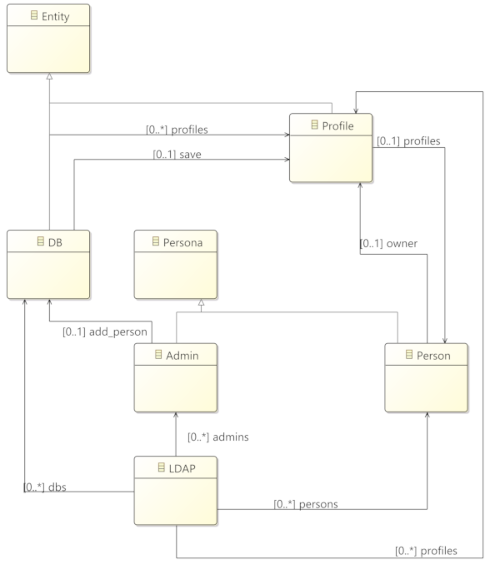
\includegraphics[scale=0.5]{henshin_class_model}
\caption{Henshin Class Model LDAP}\label{fig:henshin_model}
\end{figure}
\begin{figure}
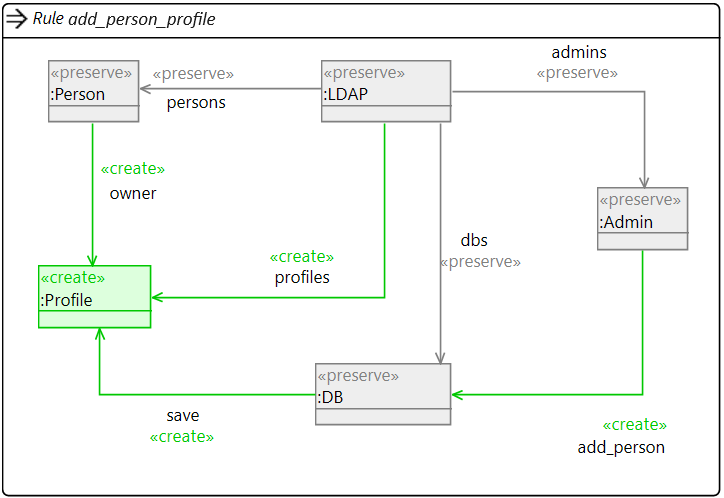
\includegraphics[scale=0.5]{henshin_rule_add_person}
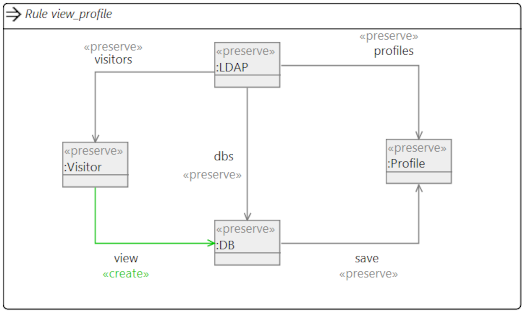
\includegraphics[scale=0.5]{henshin_rule_view_profile}
\caption{Illustrated rules in Henshin: view\textunderscore{profile} rule related to $US_2$ and add\textunderscore{person} related to $US_1$}\label{fig:henshin_rule}
\end{figure}
\begin{figure}
\center
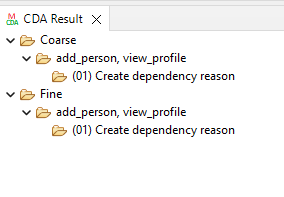
\includegraphics[scale=0.5]{henshin_cpa_result}
%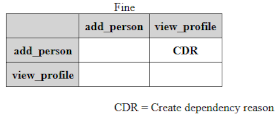
\includegraphics[width=8.13cm, height=3.6cm]{henshin_result}
\caption{Henshin CDA result visualises dependencies between user stories}\label{henshin_cpa_result}
\end{figure}
\end{example}
\begin{example}
Looking at the USs mentioned in the example \ref{example_conflict}, $US_1$: \enquote{As a user, I am able to edit any landmark.} and $US_2$:\enquote{As a user, I am able to delete only the landmarks that I added.}. First, we minimize $US_1$ and divided it into three USs as follows:
\begin{itemize}
\item $US_1a$:\enquote{As a user, I am able to add any landmark.}
\item $US_1b$:\enquote{As a user, I am able to modify any landmark.}
\item $US_1c$:\enquote{As a user, I am able to delete any landmark.}
\end{itemize}
Figure \ref{fig:conflict_model} shows the class model \enquote{Map} while figure \ref{fig:conflict_rule} shows the defined rules in Henshin, with each rule corresponding to a user story.

In this example, we assume that a user only performs one action at a time.
If $US_1c$ is translated into a rule and then CDA (Conflict and Dependency Analysis) is applied (Figure \ref{fig:conflict_cda}), Henshin would find a \enquote{Delete-Delete} conflict between two \enquote{Actions (verbs)} in $US_1c$ and $US_2$ where two users are allowed to delete the same landmark. This conflict can be avoided if $US_1c$ is replaced with $US_2$, as two users are then no longer allowed to delete the same landmark.

Figure \ref{fig:conflict_cda} shows the conflicts and dependencies between two rules. For Instance, there is a \enquote{Create-Delete} conflict between $US_1b$ and $US_2$. If the specific landmark are deleted, $US_1b$ cannot modify that landmark anymore.
%The CDA is also able to recognise inconsistencies between user stories. The inconsistency for example between $US_1c$ and $US_2$ can be recognised because the corresponding rules also have a \enquote{Delete-Delete} conflict. This occurs when the same landmark is deleted. %However, we are investigating the extent to which inconsistencies can be recognised at all. That would be another open question.

\begin{figure}[h]
\center
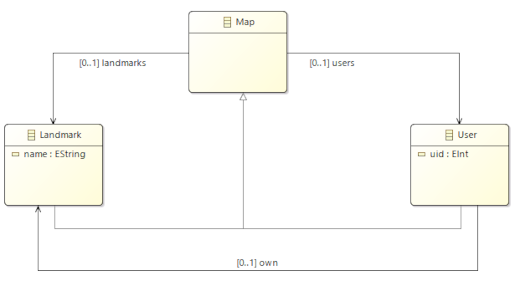
\includegraphics[scale=0.5]{henshin_conflict_model}
\caption{Henshin Class Model Map}\label{fig:conflict_model}
\end{figure}
\begin{figure}[h]
\center
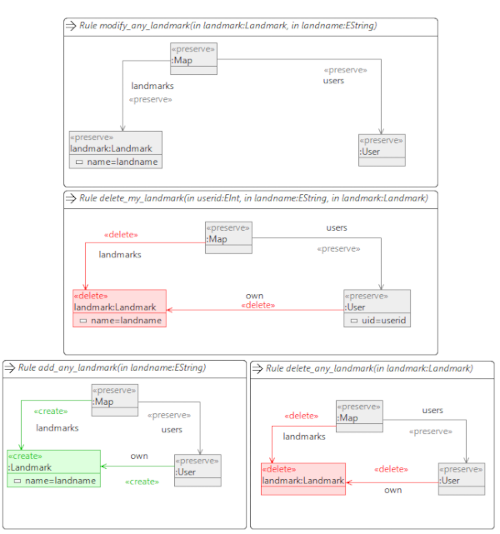
\includegraphics[scale=0.7]{henshin_conflict_rule}
\caption{Illustrated rules in Henshin: add\textunderscore{any}\textunderscore{landmark} rule related to $US_1a$, modify\textunderscore{any}\textunderscore{landmark} rule related to $US_1b$, delete\textunderscore{any}\textunderscore{landmark} rule related to $US_1c$  and delete\textunderscore{my}\textunderscore{landmark} rule related to $US_2$ }\label{fig:conflict_rule}
\end{figure}
\begin{figure}[h]
\center
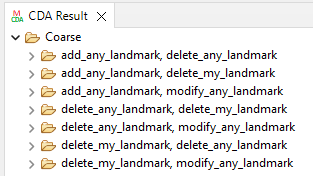
\includegraphics[scale=0.5]{henshin_conflict_cda_result}
\caption{Henshin CPA result visualises conflicts and dependencies between user stories}\label{fig:conflict_cda}
\end{figure}
\end{example}

%\begin{example}
%To demonstrate the main idea of refactoring in Henshin Born et al. represent an example for class modeling limited to one rule \cite{born2016algorithm}. Rule \emph{Move\_Attribute} (Figure \ref{fig:henshin_refractoring_rule} (a)) specifies the shift of an attribute from its owning class to an associated one along a reference. It is shown in abstract syntax. Objects and references tagged by \emph{\texttt{<<preserve>>}} represent unchanged model elements, elements tagged by \emph{\texttt{<<create>>}} represent new ones whereas those tagged by \emph{\texttt{<<delete>>}} are removed by the transformation \cite{mens2007analysing}.


%\begin{figure}
%\center
%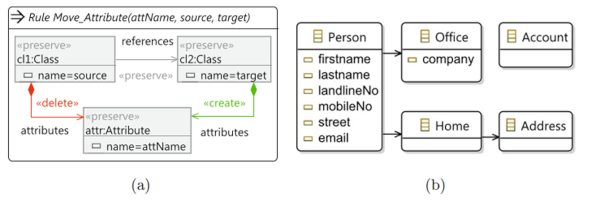
\includegraphics[width=14.13cm, height=5.0cm]{Henshin_refactoring_rule }
%\caption{Henshin refactoring rule (a) and class model Address Book (b) \cite{mens2007analysing} }\label{fig:henshin_refractoring_rule}
%\end{figure}
%Modifying the class model in Figure \ref{fig:henshin_refractoring_rule}(b) by the refactoring specified in Figure \ref{fig:henshin_refractoring_rule}(a), Born et al. observe two potential problems: (1) the attribute \emph{landlineNo} of class Person can be shifted to either class Home or class \emph{Office} (by refactoring\emph{ Move\_Attribute}) \cite{mens2007analysing}. However, if it is shifted to class Home the other refactoring becomes inapplicable (and vice versa). This means, refactoring \emph{Move\_Attribute} is in conflict with itself. (2) The attribute street of class \emph{Person} can be shifted to class \emph{Address} via class \emph{Home} (by two applications of\emph{ Move\_Attribute} along existing references). The second shift is currently not possible since class \emph{Home} does not have an attribute so far, i.e., refactoring Move\_Attribute may depend on itself. Graph transformation theory allows us to analyze such conflicts and dependencies at specification time by relying on the idea of the CPA \cite{mens2007analysing}.
%\end{example}
\subsection*{CPA Tool}
The provided CPA extension of Henshin can be used in two different ways: Its application programming interface (API) can be used to integrate the CPA into other tools and a user interface (UI) is provided supporting domain experts in developing rules by using the CPA interactively \cite{mens2007analysing}.

After invoking the analysis, the rule set and the kind of critical pairs to be analyzed have to be specified. Furthermore, options can be customized to stop the calculation after finding a first critical pair, to ignore critical pairs of the same rules, etc. The resulting list of critical pairs is shown and ordered along rule pairs. 

%Figure \ref{fig:cpa_result} depicts an example for the analysis of rule \emph{Move\_Attribute}, in which the\emph{ delete/use conflict} (1) corresponds to the example illustrated in figure \ref{fig:minimal_model} \cite{mens2007analysing}.
%The subsequent dependency results differ in their target of the second attribute movement. The first produce/use-dependency (2) represents the case of moving the attribute back to the original class, which leads to a smaller minimal model with only two classes referencing each other, as depicted in Figure \ref{fig:minimal_model}. The highlighting by enclosing hash marks is the
%most important information, since the enclosing element is the cause of the dependency. The link between 2:Class and 3:Attribute is created by the first rule application and is required by the second application. Since all elements and values in the minimal model may be matched by the first and the second rule application, there is a generic approach to represent attribute
%values. Value \emph{r1\_source\_r2\_target}, e.g., means that it must conform to value source in rule \emph{r1} and value target in rule \emph{r2}, respectively (compare Fig. \ref{fig:henshin_refractoring_rule}(a)).

%The second dependency reported in Figure \ref{fig:cpa_result} is the handling of two consecutive attribute shifts.

%\begin{figure}
%\center
%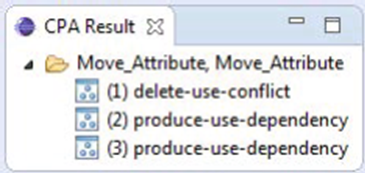
\includegraphics[width=6.22cm, height=2.96cm]{cpa_result}
%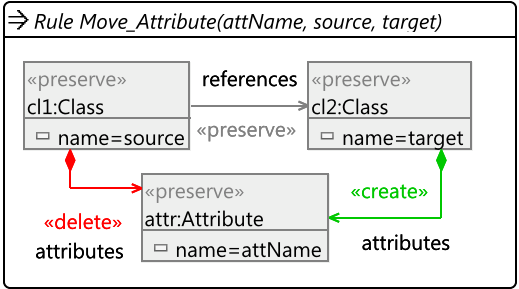
\includegraphics[width=6.22cm, height=2.96cm]{rule_move_attribute}
%\caption{The result view\cite{born2015analyzing} }\label{fig:cpa_result}
%\end{figure}
%\begin{figure}
%\center
%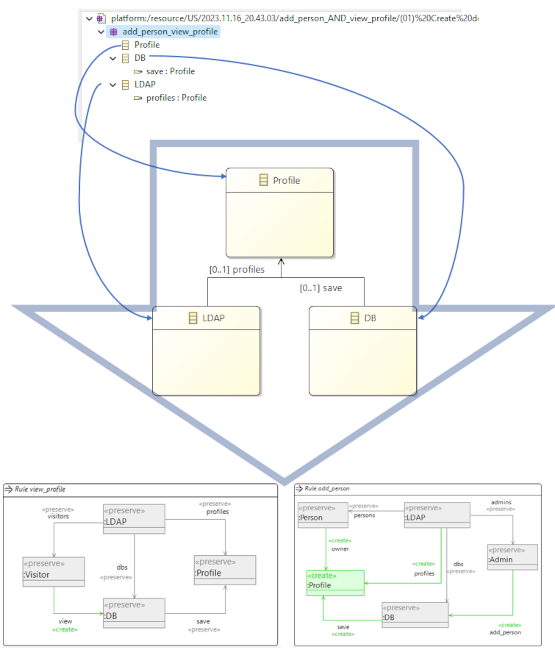
\includegraphics[width=12.13cm, height=13.0cm]{detailed_representation}
%\caption{Detailed representation of a critical pair showing a dependency \cite{born2015analyzing} }\label{fig:minimal_model}
%\end{figure}

\subsection*{Conclusion}\label{henshin_groove_conclusion}
It is notable that Henshin's critical pair analysis (CPA) remains agnostic to the specifics of instance graphs. Consequently, model checking in Henshin merely requires the set of rules. In the Henshin approach, instance graphs are not explicitly selected; instead, only rule pairs are analysed, considering conflicts and dependencies.

Since Henshin enables the specification of constraints and conditions within rules, which can be useful for enforcing and verifying US requirements to ensure that constraints are met.

Moreover, a compelling factor in favor of Henshin is the inherent support of a versatile \emph{application programming interface} (API) by the CPA extension, facilitating seamless integration of CPA functionality into various tools, including Java-based platforms.



